\documentclass[12pt, a4paper]{report}
%\usepackage{ragged2e}
\usepackage[T1]{fontenc}
\usepackage{pgf}
% \usepackage[condensed,math]{kurier}
% \usepackage[T1]{fontenc}
\usepackage{svg}
\usepackage{tikz}
\usepackage{stanli}
\usepackage{afterpage}
\usepackage{multirow}
\usepackage{subfig}
\usepackage{pgfpages}
\usepackage{svg}
\usepackage{rotating}

\usepackage{scalefnt}
\usepackage{placeins}
\usepackage{enumitem}
\usepackage{float}

% COMMANDS
\newcommand*\circled[1]{\tikz[baseline=(char.base)]{
            \node[shape=circle,draw,inner sep=2pt, fill=white] (char) {#1};}}

\pgfpagesdeclarelayout{boxed}
{
	\edef\pgfpageoptionborder{0pt}
}
{
	\pgfpagesphysicalpageoptions
	{%
		logical pages=1,%
	}
	\pgfpageslogicalpageoptions{1}
	{
		border code=\pgfsetlinewidth{2pt}\pgfstroke,%
		border shrink=\pgfpageoptionborder,%
		resized width=.9\pgfphysicalwidth,%
		resized height=.9\pgfphysicalheight,%
		center=\pgfpoint{.5\pgfphysicalwidth}{.5\pgfphysicalheight}%
	}%
}

\pgfpagesuselayout{boxed}

% Language setting
% Replace `english' with e.g. `spanish' to change the document language
\usepackage[french]{babel}

% Set page size and margins
% Replace `letterpaper' with `a4paper' for UK/EU standard size
\usepackage[a4paper,top=2cm,bottom=1.5cm,left=1.5cm,right=1.5cm,marginparwidth=1.75cm]{geometry}

% Useful packages
\usepackage{amsmath}
\usepackage{graphicx}
\usepackage[colorlinks=true, allcolors=black]{hyperref}
\usepackage{titletoc}
\usepackage{titlesec}
\usepackage{lipsum}
\usepackage{tikz}
\usepackage{tikz-uml}

\titlespacing*{\section}{0pt}{5.5ex plus 1ex minus .2ex}{4.3ex plus .2ex}

% COMMAND FOR DETAILED USECASE LIST
\newcommand{\DetailedUsecases}[1]{%
    \foreach \title in {#1}{%
        \subsection{Cas <\title>}
			\vspace{12px}
			\begin{center}
				\FloatBarrier
				\begin{figure}[H]
				\begin{center}
					\input{diag tables/\title}
				\end{center}
				\caption{Fiche descriptive de Cas <\title>}
				\label{fig:fiche \title}
				\end{figure}
				\vspace{20px}
				\FloatBarrier
				\begin{figure}[H]
				\begin{center}
				\begin{tikzpicture} 
					\input{diag seq/\title}
				\end{tikzpicture}
				\end{center}
				\caption{Diagramme de séquence système de Cas <\title>}
				\label{fig:seq \title}
				\end{figure}
			\end{center}
    }%
}

% COMMAND FOR DETAILED SEQUENCE SYSTEM DIAGRAMS
\newcommand{\DetailedSeqDiag}[1]{%
    \foreach \title in {#1}{%
        \subsection{Diagramme de Cas <\title>}
			\vspace{12px}
			\begin{center}
				\FloatBarrier
				\begin{figure}[H]
				\begin{center}
				\begin{tikzpicture} 
					\input{diag det seq/\title}
				\end{tikzpicture} 
				\end{center}
				\caption{Diagramme de séquence système detaillé de cas <\title>}
				\label{fig:seqdet \title}
				\end{figure}
			\end{center}
    }%
}

\begin{document}
	
	
\begin{titlepage}
    \begin{center}
        \vspace*{0.6cm}
        
        % University logo and faculty name
        
\includegraphics[width=0.18\textwidth]{images/university_logo.png}
        \vspace{0.1cm}
        
        % Titles for faculty, department, and university name
        {\large Université Constantine 2} \par
        {\large Faculté NTIC, Département IFA } \par
        
        \vspace{1cm}

        \Huge
        \textbf{MINI PROJET GL}
        
        \vspace{2cm}
        
        \Huge
        % Tourniquet image
        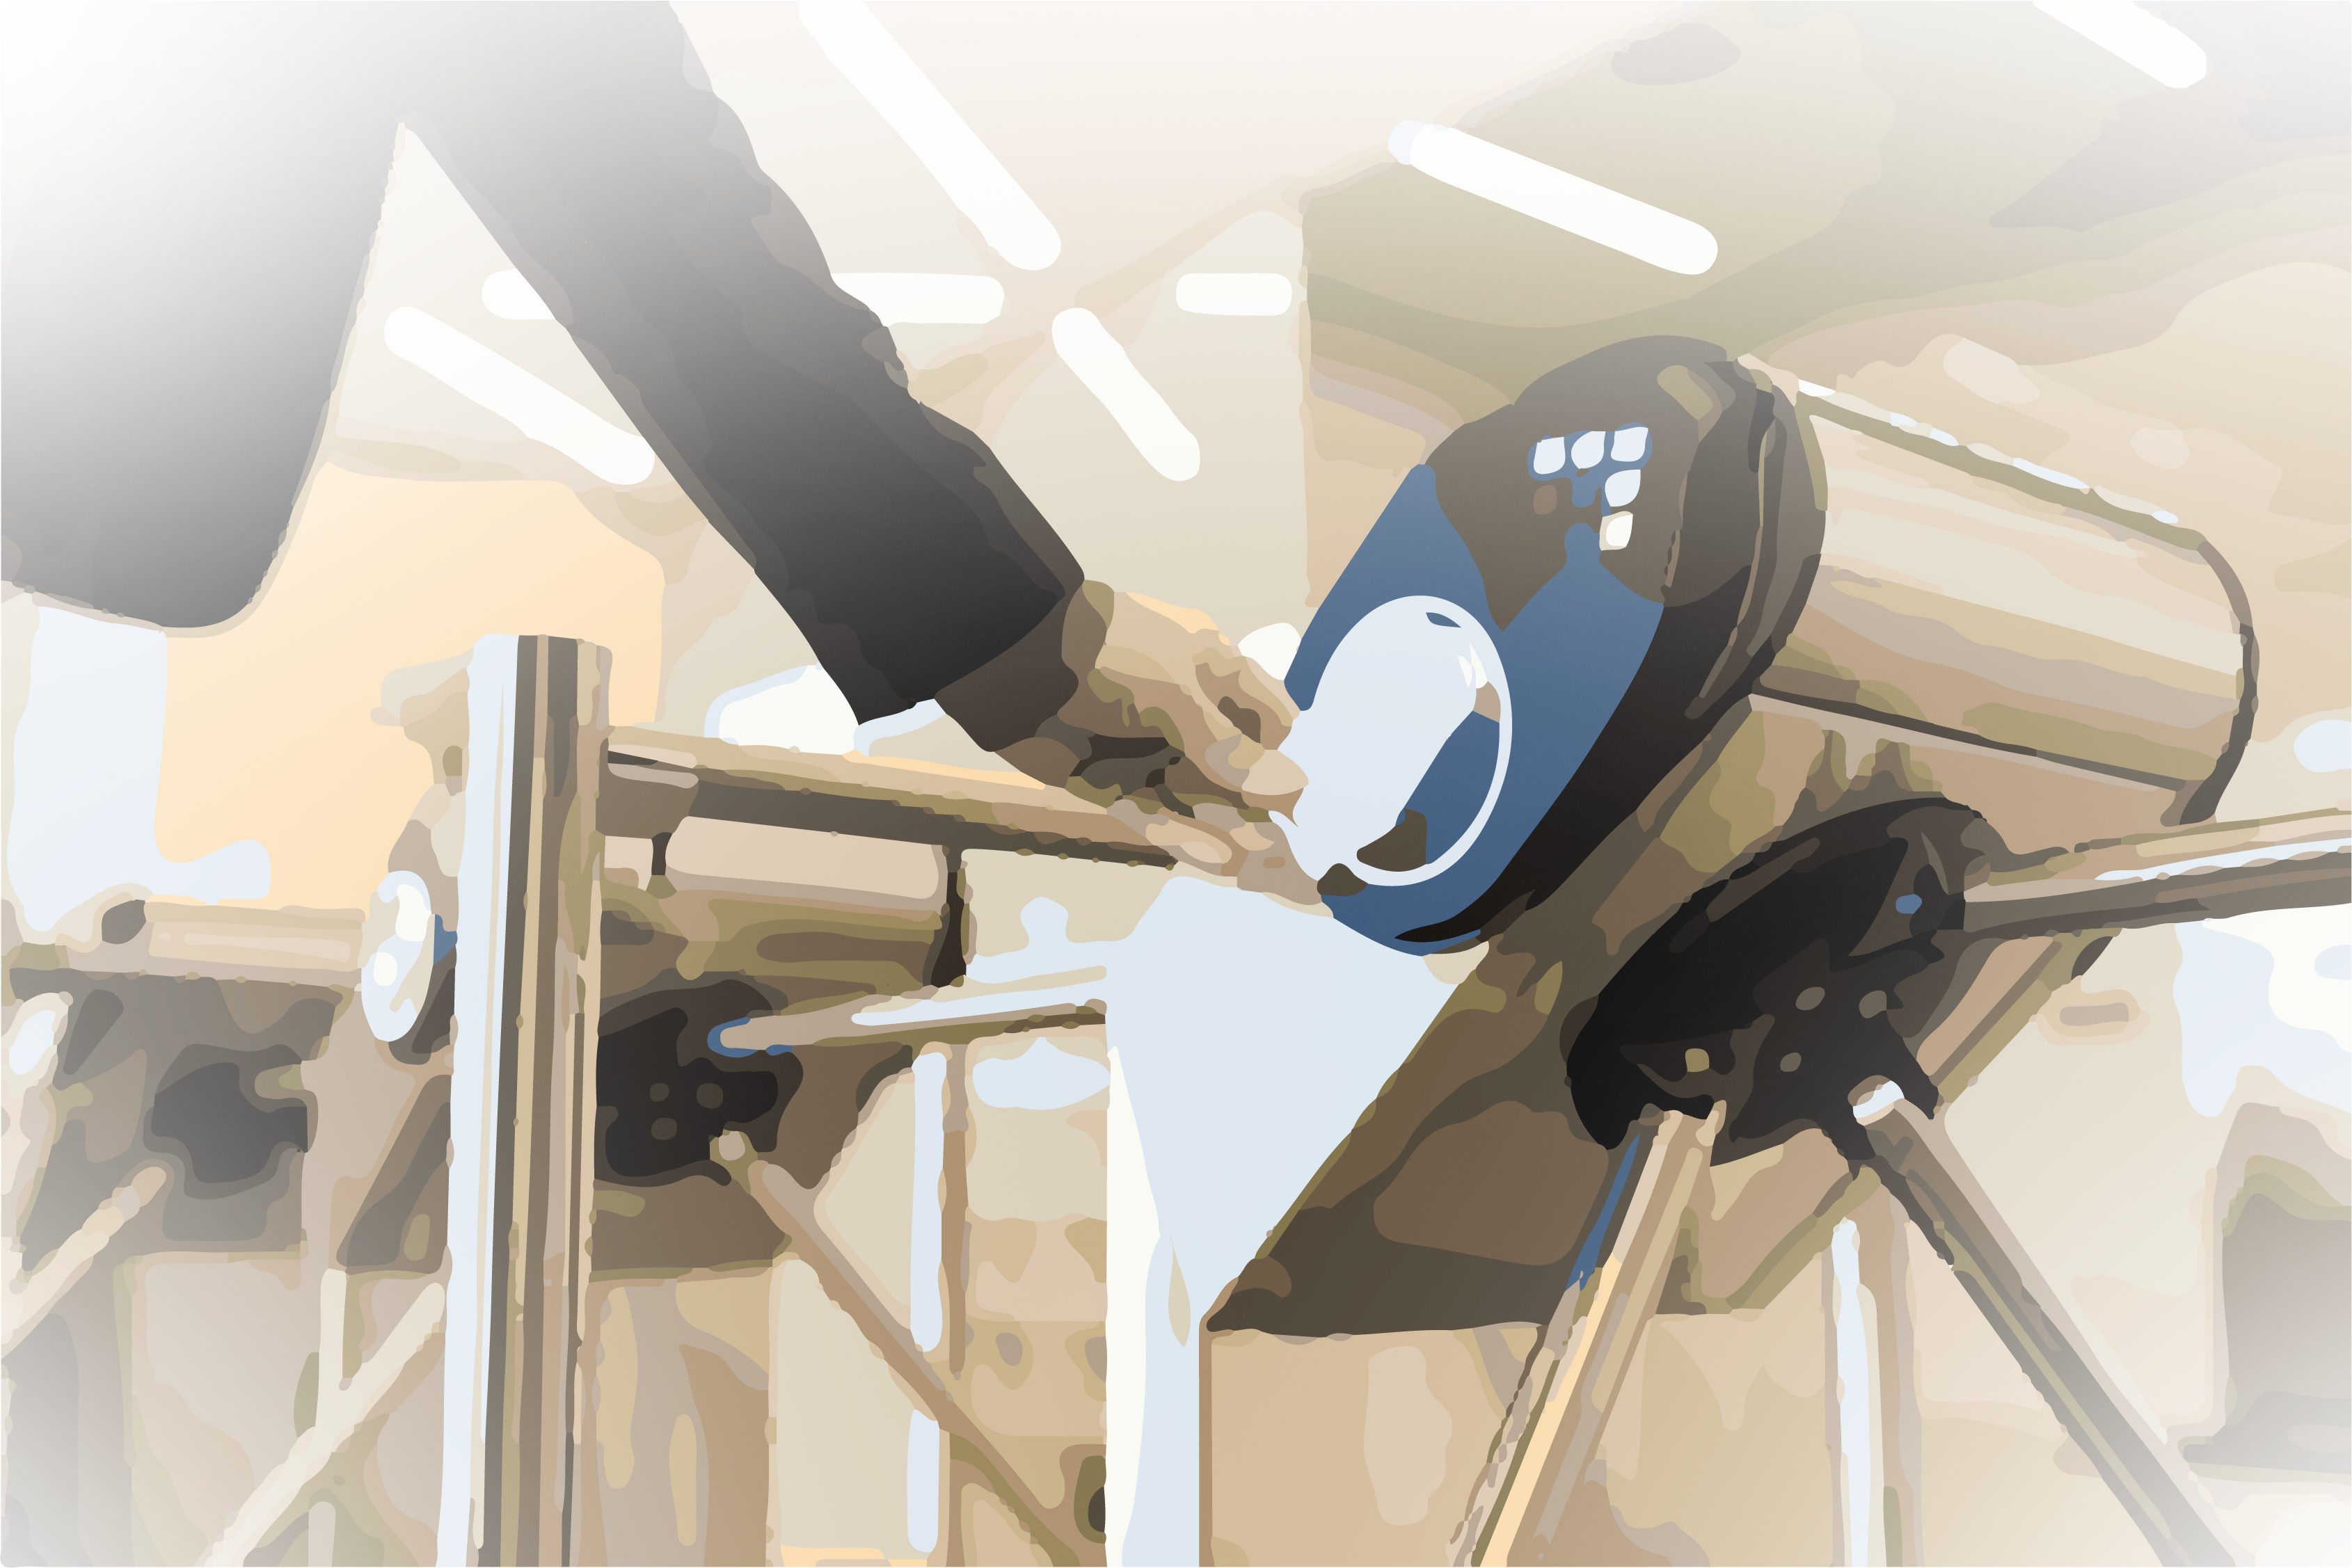
\includegraphics[width=0.7\textwidth]{images/tourniquett.png}
        
        \vspace{4.2cm}	
        
    \end{center}

    \Large
    \begin{tabbing}
        \hspace*{1em}\= \hspace*{8em} \= \kill % set the tabbings
        \> Membres:\>  \textbf{YAHIA BOUDAH (G01)} \\
        \> Module:\>  GL  \\
        \> Année Univ: \> 2023-2024 \\
        \> Date de Soum: \>  01.01.2024 \\
        \> Supervisé par: \> Dr. Kermani
    \end{tabbing}
    
\end{titlepage}

	\newpage
	\begin{center}
		\vspace*{\fill}
		\vspace*{\fill}
		
\includegraphics[width=500px]{images/bismillah.png}
		\vspace*{\fill}
		\vspace*{\fill}
	\end{center}
	\newpage
	\begin{center}
		% \centering
		\vspace*{\fill}
		\vspace*{\fill}
		{\Huge\bfseries Contrôle d'Accès Physique par Tourniquets Tripodes avec Codes QR\par}
		\vspace*{\fill}
		\vspace*{\fill}
	\end{center}
	
	
	% \titlecontents{section}[0pt]{\large\bfseries}{\thecontentslabel\hspace{1em}}{}{\titlerule*[8pt]{.}\contentspage}

	\tableofcontents

	%\justifying
	\scalefont{1.2}
	
	\chapter{Introduction}
	
\section{Présentation}
\raggedright\setlength{\parindent}{1em}
Dans un environnement universitaire dynamique, la gestion efficace des accès devient une nécessité. Ce projet vise à introduire un système de contrôle d'accès physique aux entrées de l'université, en utilisant des tourniquets tripodes et des codes QR. Ce système implique deux types d'employés: un agent et un administrateur. L'université doit faire face à diverses difficultés concernant la sécurité et la gestion des entrées. Parmi celles-ci, la nécessité de prévenir les entrées répétées avec le même code QR, d'organiser les entrées de manière structurée et de limiter l'accès exclusivement aux membres de l'université.
\newline
\newline
Notre objectif dans ce document est de réaliser une solution en utilisant la méthodologie UML. Le processus est simple: un membre de l'université présente son code QR au tourniquet, qui le scanne pour valider l'accès. Si le code est valide, l'entrée est autorisée, sinon elle est refusée. Les membres ont l'option de demander de l'assistance à l'agent pour entrer si ils ont oublié leur code, ou si leur code ne marche pas. Ils ont aussi l'option de mettre à jour leur code s'ils soupçonnent que quelqu'un a volé une version de leur code.
Notre agent attrape les entrants illégaux lorsqu'ils tentent de sortir et les oblige à payer une amende. L'admin peut réaffecter les agents à différentes portes et contrôler les tourniquets.
\newline
\newline
En adoptant ce système, nous visons à renforcer la sécurité, à organiser les entrées et à garantir que seuls les membres de l'université bénéficient d'un accès autorisé.
\newline
\newline
Ce projet a connu de nombreuses itérations, présentées dans la conclusion du projet.
	\pagebreak
	
	\chapter{Expression des Besoins}
	

\section{Modèle de spécification}
    
    \begin{description}
        \item[Acteurs] \hfill \\
            Les acteurs qui interagissent avec notre système global sont:
            \vspace{8px}
            \begin{description}
                \item[\textcolor{red}{Primaires}] \hfill \\ \textbf{Personne} (Passeur ou Visiteur) \\ \textbf{AgentP} signifie "AgentPorte"
                \vspace{8px}
                \item[\textcolor{magenta}{Secondaires}] \hfill \\ \textbf{<<Sys>> Logiciel} (Interagit avec autres sous-systèmes)\\ \textbf{AdminP} signifie AdministrateurPortes
            \end{description}
        
        \vspace{8px}
        \item[Besoin Fonctionnelles] \hfill \\
            \begin{itemize}[label=•]
                \item Passage (Entrée ou Sortie) autorisée des membres d'université par la tourniquet.
                \item Service d'assistance à l'entrée assuré par l'agent de porte.  
                \item L'attrape des visiteurs illégaux lorsqu'ils tentent de sortir et la collection des amendes.
                \item Facilitation pour les membres de mettre à jour leur code QR s'ils soupçonnent que quelqu'un possède la version actuelle de leur code. 
            \end{itemize}
        \vspace{8px}
        \item[Besoin non Fonctionnelles] \hfill \\
            \begin{itemize}[label=•]
                \item Disposer d'une interface intuitive et rapide pour l'agent de porte afin de faciliter ses tâches quotidiennes.
                \item Avoir un système robuste toujours connecté.
                \item Avoir un administrateur capable d'affecter des agents à différentes portes et de gérer les tourniquets
            \end{itemize}
    \end{description}
    \pagebreak


	

\section{Modèle de cas d'utilisation}
    \subsection{Diagrammes de cas d'utilisation}
    Notre système global complet est composé de quatre sous-systèmes:
    \begin{description}
        
        \item[Système Tourniquet] implique les tourniquets placés aux portes de l'université
        \item[Système AgentP] implique l'agent de porte qu assiste les gens à entrer ou sortir 
        \item[Système Logiciel] L'interface utilisée par l'agentP, les membres et l'adminP
        \item[Système Imprimante] Pour imprimer des codes QR en cas d'urgence


    \end{description}
    \vspace{8px}
    
    Ceux-ci peuvent être classés en deux catégories principales :\linebreak 
    \begin{enumerate}
        \item \textbf{Partie Passage} qui implique le système de Tourniquet et le système AgentP, utilisés seulement par l'acteur Personne. Présentée dans la figure \ref{fig:syspart1}
        \linebreak
        \item \textbf{Partie Logiciel et Imprimante} qui implique les deux systèmes Logiciel et Imprimante, utilisés par tous les acteurs. Présentée dans la figure \ref{fig:syspart2}
    \end{enumerate}
    \vspace{8px}

    
\FloatBarrier
\begin{figure}[H]
%\centering
\begin{tikzpicture}

    \begin{scope}[local bounding box=boundingbox]
    
        % Turnstile system
        \begin{umlsystem}[x=-4]{Système Tourniquet}
            
            
            %1 Passer
            \umlusecase[fill=red!30]{ 
                Passer
            }

            %2 Entrer
            \umlusecase[x=4, y=1, fill=red!30]{Entrer}
            %3 Sortir
            \umlusecase[x=4, y=-1, fill=red!30]{Sortir}

            \umlinherit{usecase-2}{usecase-1}
            \umlinherit{usecase-3}{usecase-1}
        \end{umlsystem}


        % AgentP system
        \begin{umlsystem}[x=-4, y=-5]{Système AgentP}
            
            %4 Demander
            \umlusecase[fill=orange!30]{Demander}

            % Demander Entrée
            %5 Demander Entrée
            \umlusecase[x=3, fill=orange!30]{Entrée}
            %6 Dem Entrée Sans Code
            \umlusecase[x=6.5, y=0, fill=orange!30]{Sans Code} 
            %7 Dem Entrée Avec Code
            \umlusecase[x=6.5, y=-1.5, fill=orange!30]{Avec Code}
            
            % Demander Sortie
            %8 Demander Sortie
            \umlusecase[x=3, y=-1.5, fill=orange!30]{Sortie}
            
            % Payer l'amende
            %9 Payer l'amende
            \umlusecase[x=6.5, y=-3, fill=orange!30]{Payer l'amende}

            \umlinherit{usecase-5}{usecase-4}
            \umlinherit{usecase-8}{usecase-4}
            \umlinherit{usecase-6}{usecase-5}
            \umlinherit{usecase-7}{usecase-5}
            % include Pay Fine
            \umlinclude{usecase-8}{usecase-9}
            \draw [->, dashed] (usecase-6) .. controls +(3,-0.5) and +(2.5,0.5) .. (usecase-9) node[midway, below] {<<include>>};
            % \umlinclude{usecase-5}{usecase-8}
            
        \end{umlsystem}

        % INTER SYSTEMS ASSOC
        \draw [->, dashed] (usecase-7) .. controls +(5.5,4.5) and +(2.5,0.5) .. (usecase-2) node[midway, below] {<<extends>>};
        \draw [->, dashed] (usecase-8) .. controls +(-2.1,1.8) and +(-1.9,0.3) .. (usecase-3) node[midway, below] {<<extends>>};
        
    \end{scope}

    % ACTORS
    \umlactor[x=-9, y=-1, scale=2]{Personne}
    
    % ASSOCIATIONS
    \umlassoc{Personne}{usecase-4}
    \umlassoc{Personne}{usecase-1}

    % BOUDNING BOX
    \draw ([shift={(-0.5,-0.5)}] boundingbox.south west) rectangle ([shift={(0.5,0.5)}] boundingbox.north east);
    \node[above] at (boundingbox.north) {Système Contrôle d'Accès: Partie 1};
\end{tikzpicture}
\caption{Système Contrôle d'Accès: Partie 1}
\label{fig:syspart1}
\end{figure}
    

\FloatBarrier
\begin{figure}[H]
%\centering
\begin{tikzpicture}
    
    \begin{scope}[local bounding box=boundingbox]

        % Software system
        \begin{umlsystem}[x=-4.7]{Système Logiciel}
            
            %10 Assister
            \umlusecase{Assister}
            %11 Identifier
            \umlusecase[x=5]{Identifier}
            %12 Avec ID
            \umlusecase[x=8]{AvecID}
            %13 Avec Code
            \umlusecase[x=8, y=-1]{AvecCode}

            %14 Update Code
            \umlusecase[x=0.3, y=-2.5, width=1.1cm]{Update Code}
            %15 Imprimer Code
            \umlusecase[x=5, y=-2.5, width=1.3cm]{Imprimer Code}

            %16 Voir Profile
            \umlusecase[y=-5, width=1.3cm]{Voir Profile}

            %17 Gestion Tourniquets
            \umlusecase[x=8, y=-7, width=2.5cm]{Gestion Tourniquets}
            %18 Alumer
            \umlusecase[x=8, y=-9.5]{Changer État}

            %19 Gestion AgentP
            \umlusecase[x=3, y=-7, width=1.5cm]{Gestion AgentP}
            %20 Modifier AP
            \umlusecase[x=3, y=-9.5]{Modifier}

            % LINKS
            \umlinclude{usecase-10}{usecase-11}
            \umlinherit{usecase-12}{usecase-11}
            \umlinherit{usecase-13}{usecase-11}

            \umlinclude[name=incl]{usecase-14}{usecase-15}
            \umlextend{usecase-14}{usecase-11}
            \umlextend{usecase-15}{usecase-11}

            \umlextend{usecase-18}{usecase-17}
            %\umlextend{usecase-19}{usecase-17}
            \umlextend{usecase-20}{usecase-19}

        \end{umlsystem}

        % Printer system
        \begin{umlsystem}[x=0, y=-13]{Système Imprimante}
            %22 Impression
            \umlusecase[fill=yellow!30]{Impression}
        \end{umlsystem}
    
    \end{scope}

    % NOTES
    \umlnote[x=1, y=-4.7]{incl-1}{Seulement si le cas est utilisé par AgentP}

    % ACTORS
    \umlactor[x=-9, y=-1, scale=2]{Personne}
    \umlactor[x=-9, y=-5, scale=2]{AgentP}

    \umlactor[x=8.3, y=-5, scale=2]{AdminP}
    \umlactor[x=8.3, y=-11, scale=1.5]{<<Sys>> Logiciel}
    
    % ASSOCIATIONS
    \umlassoc{Personne}{usecase-14}
    \umlassoc{Personne}{usecase-16}

    \umlassoc{AgentP}{usecase-10}
    \umlassoc{AgentP}{usecase-16}
    \umlassoc{AdminP}{usecase-17}
    \umlassoc{AdminP}{usecase-19}

    \umlassoc{<<Sys>> Logiciel}{usecase-21}

    % BOUDNING BOX
    \draw ([shift={(-0.5,-0.5)}] boundingbox.south west) rectangle ([shift={(0.5,0.5)}] boundingbox.north east);
    \node[above] at (boundingbox.north) {Système Contrôle d'Accès: Partie 2};

\end{tikzpicture}
\caption{Système Contrôle d'Accès: Partie 2}
\label{fig:syspart2}
\end{figure}

    \begin{description}
        \item[Liste des cas d'utilisations à étudier] \hfill \\
        \item[] \begin{minipage}[t]{0.5\textwidth}
            \begin{enumerate}
                \item Passer Entrer
                \item Passer Sortir
                \item Dem Ent SansCode
                \item Dem Ent AvecCode
                \item Dem Sortie
                \item Payer Amende
                \item Assiter
            \end{enumerate}
        \end{minipage}
        \hfill
        \begin{minipage}[t]{0.4\textwidth}
            \begin{enumerate}
                \setcounter{enumi}{7}
                \item Identifier AvecID
                \item Identifier AvecCode
                \item Update Code
                \item Imprimer Code
                %\item Voir Profile
                \item Gestion tourniquet
                %\item Changer État TQ
                \item Gestion AgentP
                %\item Modifier AP
                \item Impression
            \end{enumerate}
        \end{minipage}
    \end{description}
    \pagebreak
	

\section{Étude détaillée des cas d'utilisation}
    
    \DetailedUsecases{
        Passer Entrer,
        Passer Sortir,
        Dem Ent SansCode,
        Dem Ent AvecCode,
        Dem Sortie,
        Payer Amende,
        Assister,
        Identifier AvecID,
        Identifier AvecCode,
        Update Code,
        Imprimer Code,
        %Voir Profile,
        Gestion Tourniquet,
        Gestion AgentP,
        Impression
    }
	\pagebreak

	\chapter{Analyse et Conception}
	
\section{Diagrammes de classes}
    \subsection{Diagramme de classes d'Entité}
        \FloatBarrier
        \begin{figure}[H]
        \begin{center}
            \input{diag class/entity}
        \end{center}
        \caption{Diagramme de classes d'Entité}
        \label{fig:classentity}
        \end{figure}
        \subsection{Diagrammes de classes de Contrôle}
        \FloatBarrier
        \begin{figure}[H]
        \begin{center}
            \input{diag class/control}
        \end{center}
        \caption{Diagramme de classes de Contrôle}
        \label{fig:classcontrol}
        \end{figure}
    \subsection{Diagrammes de classes Participants}
        \FloatBarrier
        \begin{figure}[H]
        \begin{center}
            \input{diag class/participant}
        \end{center}
        \caption{Diagramme de classes Participants}
        \label{fig:classpart}
        \end{figure}
	

\section{Diagrammes du séquence système detaillés}

    \DetailedSeqDiag {
        Passer Entrer,
        Passer Sortir,
        Dem Ent SansCode,
        Dem Ent AvecCode,
        Dem Sortie,
        Payer Amende,
        Assister,
        Identifier AvecID,
        Identifier AvecCode,
        Update Code,
        Imprimer Code,
        %Voir Profile,
        Gestion Tourniquet,
        Gestion AgentP,
        Impression
    }
	
\section{Diagramme du modèle relationnel}
    \FloatBarrier
    \begin{figure}[H]
    \begin{center}
        % FIGURE GOES HERE
        % ===============
        % ===============
    \end{center}
    \caption{Diagramme du modèle relationnel}
    \label{fig:classentity}
    \end{figure}
	\pagebreak

	\chapter{Conclusion}
	

TODO
\section{Étape Post-UML}
    TODO
\section{Itérations du mini projet}
    \subsection{Itération Nº1}

        \textbf{\textit{Entités Générales}}
        \vspace{8px}
        \linebreak
        Université; Personne; Tourniquet; Porte; CodeQR;
        Enseignat, Etudiant, Staff (sous-entités de Personne);Alerte; TypeAlerte; AgentSupportTechnique, AgentSécurité (sous-entités de AgentTourniquet); Passage (Entrée ou Sortie); SalleSurveillance; Imprimante; ScannerQRCode; OrdinateurSalleSurveillance
        \linebreak

        \textbf{\textit{Scénario Principal}}
        \vspace{8px}

        \begin{itemize}
            \item Une personne entre à l'université par une porte équipée de tourniquets. Il présente sa carte ou son QR CODE via une application universitaire.
            \item Le tourniquet vérifie la validité du code. Si valide, l'entrée est autorisée ; sinon, une alerte est déclenchée.
            \item L'agent technique informe l'agent sécurité du nombre de tourniquet concerné.
            \item L'agent de sécurité amène une personne dans la salle de surveillance
            \item Si l'alerte est: CodeInconnu, donc l'agent de sécurité retire la personne de l'entrée.
            \item Si l'alerte est: CodeAncien, l'agent technique vérifie si c'est la meme personne, si c'est le cas il lui imprime le code le plus récent. Sinon la personne est retirée.
            \item Si l'alerte est de type: CodeRépété. Si c'est pas la meme personne dans le système, la personne est retirée, puis l'agent technique met à jour le code de Personne propriétaire de code, et le notifie que son code a été utilisé par quelqu'un d'autre. Si c'est la meme personne, donce son code est mis à jour, et imprimé pour son entrée.
            \item Si le visiteur oublie sa carte ou n'a pas l'application, il se rend à la salle de surveillance.
            \item L'agent technique vérifie l'identité du visiteur dans la base de données. S'il est membre de l'université, un QR CODE temporaire est imprimé pour lui permettre l'accès moyennant une amende.
            \item En sortant, le visiteur glisse sa carte dans le tourniquet de sortie.
            \item Pour éviter les entrées multiples avec le même code QR, un suivi des entrées/sorties est effectué.
            \item Si un code déjà utilisé est scanné, l'entrée est refusée et une alerte de fraude est générée.
            \item En cas de fraude avérée, le fraudeur est expulsé et le détenteur légitime est notifié pour désactiver son ancien code QR.
        \end{itemize}

        \textbf{\textit{Limitations et Cas Particuliers}}
        \vspace{8px}

        \begin{itemize}
            \item Pendant les événements spéciaux, les portes sont ouvertes sans nécessité de code QR.
            \item La police, les pompiers ou les entités spéciales ont des accès différenciés.
            \item La principale faille est la possibilité d'utiliser le même code par plusieurs personnes.
            \item Pour améliorer la sécurité, l'authentification biométrique pourrait être envisagée.
        \end{itemize}

    \subsection{Itération Nº2}
        TODO
    \subsection{Itération Nº3}
        TODO

\section{Outils utilisés}
    TODO
	\pagebreak

	\begin{thebibliography}{999}
        
        \bibitem{iutenligne}
        IUTENLIGNE \\
        \url{https://prive.iutenligne.net/iuRxM0CThIXDIjzG/informatique/langages/kettaf/UML/01introduction/index.html}

        \bibitem{cmu}
        CMU \\
        \url{https://www.andrew.cmu.edu/course/90-754/umlucdfaq.html#ucdefinition}
    
    \end{thebibliography}

	\newpage
	\begin{center}
		\vspace*{\fill}
		\vspace*{\fill}
		
\includegraphics[width=500px]{images/hamdulillah.png}
		\vspace*{\fill}
		\vspace*{\fill}
	\end{center}
	
\end{document}